\documentclass{article}

\usepackage{amsmath}
\usepackage{amssymb}
\usepackage{amsthm}
\usepackage{cancel}
\usepackage{colonequals}

\usepackage{tikz}
\usetikzlibrary{arrows, arrows.meta}
\usepackage[shortlabels]{enumitem}

\usepackage{hyperref}

\theoremstyle{definition}
\newtheorem{prob}{Problem}
\newtheorem{sol}{Solution}
\newtheorem*{subsol}{Subsolution}
\newtheorem*{nota}{Notation}

\theoremstyle{plain}

\newcommand{\ps}[1]{\operatorname{ps}\left(#1\right)}
\newcommand{\set}[1]{\left\{#1\right\}}
\newcommand{\len}[1]{\left|#1\right|}
\newcommand{\elemp}[1]{\Pi(#1)}
\newcommand{\defeq}{\colonequals}
\newcommand{\symdiff}{\mathbin{\Delta}}
\newcommand{\Z}{\mathbb{Z}}
\newcommand{\parity}{\operatorname{parity}}
\newcommand{\Exp}[1]{\mathbb{E}\left[#1\right]}

\newcommand{\myscale}{0.75}
\newcommand{\infzz}{I\mkern-2mu Z}
\newcommand{\showfrom}[1]{\text{from #1}}
\newcommand{\zz}{Z\mkern-2muZ}


\title{\textsc{Math puzzles}}

\author{Charles Kolozsvary}
\date{\today}

\begin{document}

\maketitle

\section*{Introduction}
There are a wide variety of math brain teasers out there. But most people don't have the interest or time to try to tackle involved ones. So here's a short list of bite-sized puzzles to try.\footnote{However, just because these puzzles are small does not mean they are obvious, so you definitely shouldn't be discouraged if you get stumped. Though none of the answers require any lengthy computation, so avoid going down that road.} The solution to each problem can be found in Section~\ref{appen}.

\section{Problems}
\begin{prob}
Without solving for $x$, show that if
\[
x + \frac{1}{x} = 1, \text{ then } x^7 + \frac{1}{x^7} = 1.
\]
\end{prob}

\begin{prob}
Find the smallest positive integer divisible by 15 which has exactly 15 divisors.
\end{prob}

\begin{prob}
Show that there is an element in the infinite sequence
\[
7, 77, 777, 7777, \ldots
\]
that is divisible by 2003.
\end{prob}

\begin{prob}[Harder]\label{prob:f2n}
The set $A$ consists of $n+1$ positive integers, none of which have a prime divisor greater than the $n$th smallest prime. Show that there exists a nonempty subset $B \subseteq A$ where the product of the elements of $B$ is a perfect square.\footnote{An integer is a perfect square if it is the square of another integer. I.e., $s$ is a perfect square if $s \in \set{n^2 \mid n \in \mathbb{Z}}$.}
\end{prob}

\begin{prob}
You have an $n$-sided die. What is the expected number of rolls it takes to land on each face at least once?
\end{prob}

\begin{prob}
There are $100$ light switches, all originally off. One hundred people pass by the switches; the first person flips every one, the second flips every other one, the third every third one, and so on. After the $100$th person passes, which lights are on?
\end{prob}

\begin{prob}
There are $100$ noodles. Uniformly at random, you select two noodle ends and connect them, repeating the process until there are no more ends to connect. On average, how many loops form, and what is the probability that just one loop forms? 
\end{prob}

\begin{prob}
\[
\begin{tikzpicture}[scale=\myscale]
  % Coordinates
  \coordinate (B) at (0.97, 2.22);
  \coordinate (C) at (5.97, 7.56);
  \coordinate (D) at (-3.56, 2.06);
  \coordinate (A) at (10.50, 7.72);
  \coordinate (E) at (8.90, 1.29);
  \coordinate (F) at (2.19, 8.12);
  \coordinate (G) at (4.57, 1.99);
  \coordinate (H) at (-1.70, 8.39);
  \coordinate (I) at (0.75, 12.25);

  % Drawing
  \draw[-Stealth] (C) -- (D);
  \draw[-Stealth] (B) -- (A);
  \draw (B) -- (C);
  \draw[Stealth-] (E) -- (F);
  \draw (F) -- (G);
  \draw[-Stealth] (G) -- (H);
\end{tikzpicture}
\]
What is the maximum number of regions that $n$ zig-zag lines can segment the 2D plane into? Each zig-zag is made up of a pair of half-infinite parallel lines and a finite one connecting them. $\zz_2 = 12$.
\end{prob}

\newpage

\section{Solutions}\label{appen}
\begin{sol}
Consider the powers of $x$:
\begin{align*}
x^2 &= x - 1;\\
x^3 &= x^2 - x \\
&= x - 1 - x \\
&= -1.
\end{align*}
Therefore $x^6 = {(x^3)}^2 = (-1)^2 = 1$, so $x^7 = x$.
\end{sol}

\begin{sol}
By the fundamental theorem of algebra, every positive integer can be written as a product of prime powers, $\prod_{i=1}^kp_i^{r_i}$.

It's not too hard to reason about the number of divisors of a product of powers. For each prime power we can use anywhere between 0 and all of the powers of the prime as a divisor. E.g., if our number is $81=3^4$ then we can choose zero through four ``multiplicative copies'' of $3$ as divisors of $81$. This count is independent across each prime, so
\[
\text{\# of divisors of } \prod_{i=1}^kp_i^{r_i} = \prod_{i=1}^{k}r_i+1.
\]

The factors of $15$ are only $3$ and $5$, so the least number which has $15$ divisors and divides $15$ must have a prime factorization of the form $3^a5^b$, where $a,b \geq 1$. However, the product of $a+1$ and $b+1$ \textit{must also equal} $15$ to give $15$ divisors. I.e.,
\begin{align*}
&(a+1)(b+1) = 3\times 5\\
\implies & (a = 2 \text{ and } b = 4) \text{ or } (a = 4 \text{ and } b = 2).
\end{align*}
And since we want $3^a5^b$ to be as small as possible, we put the larger power on the smaller prime, giving our final answer: $3^45^2 = 2025$.
\end{sol}
\begin{sol}
Let $a_i$ denote the $i$th element of the sequence so $a_1 = 7$, $a_2 = 77$, and so on. There are an infinite number of elements in our sequence but only a finite number of remainders when dividing any element in the sequence by 2003. So, by the pigeon hole principle, there must exist two elements $a_i \ne a_j$ which have the same remainder. That is, for $m,n \in \mathbb{Z}_+$,
\begin{align*}
a_i = m &\times 2003 + r\\
a_j = n &\times 2003 + r.
\end{align*}
Without loss of generality, suppose $a_j > a_i$. Then $a_j - a_i = (m-n) \times 2003$, so $2003$ divides $a_j - a_i$.

But $a_j - a_i$ is not an element of the sequence, so let's look at it more closely using an example. Consider $a_{9} - a_{5}$:
\begin{align*}
a_9 - a_5 &= \begin{aligned}[t] &777777777\\ -&\hphantom{0000}77777\end{aligned}\\
&= \hphantom{-} 777700000\\
&= a_4 \times 10^5.
\end{align*}
So in general $a_j - a_i$ = $a_{j-i} \times 10^i$.

Since $2003$ divides $a_{j-i} \times 10^i$, but $2003$ shares no factors with any power of $10$ (neither $2$ or $5$ divide $2003$), $2003$ must divide $a_{j-i}$.\footnote{I.e., we use the fact that if $c$ divides $ab$ and $\gcd(c,b) = 1$, then $c$ divides $a$.}
\end{sol}

\begin{sol}
\begin{nota}
Let the product of the elements of a set $S$ be denoted by $\elemp{S}$. I.e.,
\[
\elemp{S} \defeq \prod_{s \in S}s.
\]

Given a prime factorization $m = \prod_{i = 1}^n p_i^{e_i}$, where $p_i$ denotes the $i$th prime, let the ``parity signature'' of
$m$ be the bit string which records the parity of each prime exponent of $m$, denoted by $\ps{m}$. I.e., using the notation of formal language theory with alphabet $\Sigma = \set{0,1}$,
\[
\ps{m} \defeq \prod_{i = 1}^n \operatorname{parity} e_i,
\]
where
\[
\operatorname{parity} x \defeq \begin{cases} 0 & \text{if $x$ is even}\\
1 & \text{if $x$ is odd}.\end{cases}
\]
For example (if $n = 5$), $\ps{2^311^{71} = 2^33^05^07^011^{71}} = 10001$.
\end{nota}

\begin{proof}
``None of which have a prime divisor greater than the $n$th smallest prime'' is the same as ``every element of $A$ has only the first $n$ primes in it's prime factorization,'' so each $a \in A$ can be written as $\prod_{i=1}^np_i^{e_i}$.

We want to show that there exists a nonempty subset $B \subseteq A$ such that $\ps{\elemp{B}} = 0^n$.\footnote{An integer is a perfect square if and only if its parity signature is an all-zero string because if each prime exponent is even, we can factor out a $2$ from each of them, and since
$x^{ca}y^{cb} = {(x^ay^b)}^c$, $\prod_{i=1}^np_i^{2f_i} = {(\prod_{i=1}^np_i^{f_i})}^2$.} To do this, we first want to show that there exist two nonempty subsets $C,D\subseteq A$ whose element products have the same parity signature.

$\len{A} = n+1$, so there are $2^{n+1} - 1$ nonempty subsets of $A$. Let
\[
P = \set{\ps{\elemp{B}} \mid B \subseteq A \text{ and $B$ nonempty}}.
\]
Then $\len{P} = 2^{n+1} -1$ only if the parity signatures of each $\elemp{B}$ are distinct. But there are only $2^n$ unique bit strings of length $n$, and
\[
\qquad 2^{n+1} - 1 > 2^n \iff 2^n > 1 \qquad \forall n\ge 1.
\]

So, by the pigeon hole principle, there exist distinct $C, D \subseteq A$ whose element products have the same parity signature.\footnote{In other words, there are more nonempty subsets of $A$ than possible parity signatures, so at least two (distinct) nonempty subsets must produce the same parity signature.} And if
\[
\ps{\elemp{C}} = \ps{\elemp{D}},
\]
then
\begin{equation}\label{eq:perf}
\ps{\elemp{C}\times\elemp{D}} = 0^n
\end{equation}
because powers are added when numbers are multiplied, and an odd plus and odd is even, and an even plus an even is even.\footnote{Any odd plus another odd is even because $(2m + 1) + (2n + 1) = 2(m + n + 1)$.}

However,
\begin{equation}\label{eq:ne}
\elemp{C} \times \elemp{D} \neq \elemp{C \cup D}
\end{equation}
if $C \cap D \neq \emptyset$ since each member of $C \cap D$ appears twice in the product on the LHS of \eqref{eq:ne} but only once in the product on the RHS. But it's not too hard to show that if we remove the doubled members of the product from $C \cap D$ we will still be left with a perfect square. That is, we can quickly show that if $ab$ is a perfect square and $b$ is a perfect square, then $a$ is a perfect square. By definition, if $ab$ and $b$ are perfect squares, then $\exists m,n \in \Z: m^2 = ab \text{ and } n^2 = b$. So $\frac{m^2}{n^2} = a$ and thus $(\frac{m}{n})^2 = a$.

Recall from \eqref{eq:perf} that $\elemp{C}\times\elemp{D}$ is a perfect square. So
\begin{align*}
\elemp{C} \times \elemp{D} &= \elemp{C \setminus D} \times \left(\prod_{i \in C \cap D} i\right)^2 \times \elemp{D \setminus C}\\
&= \elemp{C \symdiff D} \times \left(\prod_{i \in C \cap D} i\right)^2.
\end{align*}
Therefore $\elemp{C \symdiff D}$ is a perfect square, and $C \symdiff D \subseteq A$ is nonempty since we only considered nonempty subsets of $B$ when we originally applied the pigeon hole principle.\footnote{$\symdiff$ denotes the \textit{symmetric difference} of two sets: $A \symdiff B \defeq (A \setminus B) \cup (B \setminus A) = (A \cup B) \setminus (A \cap B)$.}
\end{proof}

\begin{proof}[Alternate proof of Problem \ref{prob:f2n}] %% Mini sub proof
Since the members of $A$ are positive and have no divisor greater than the $n$th prime, we can write each $a \in A$ as
\[
a = \prod_{i=1}^n p_i^{e_i(a)},
\]
where $p_i$ is the $i$th prime and $e_i(a) \ge 0$ is the exponent of $p_i$ in the prime factorization of $a$.

Now define a map $f : A \rightarrow \mathbb{F}_2^n$ such that
\[
f(x) = (e_1(x) \bmod 2, e_2(x) \bmod 2, \dots, e_n(x) \bmod 2).
\]
Applying $f$ records the parity of the exponents of the primes in the prime factorization of $x$, and if all said parities are zero, then $x$ is a perfect square.\footnote{This is due to properties of exponentiation: since ${(x^ay^b)}^c = x^{ac}y^{bc}$, then (in reverse) $\prod_{i = 1}^np_i^{2r_i} = ({\prod_{i=1}^np_i^{r_i}})^2$.}

Now arbitrarily order the elements of $A$ such that $\set{a_1,a_2,\dots,a_{n+1}} = A$, and apply apply $f$ to each $a \in A$ to produce $n+1$ $n$-dimensional vectors, $v_1,v_2,\dots,v_{n+1}$, in $\mathbb{F}_2^n$. Since there are more vectors than the dimension of the vector space, $n$, $\set{v_1,\dots,v_j}$ must be linearly dependent, i.e., there must exist not-all-zero weights
\[
w_j \in \set{0, 1} = \mathbb{F}_2 \quad \text{for $j \in \set{1, \dots, n+1}$}
\]
such that
\begin{equation}\label{eq:zerovec}
\sum_{j=1}^{n+1} w_j v_j = \mathbf{0}.
\end{equation}

If we let $B = \set{a_j \mid w_j = 1}$, then
\[
P = \prod_{b \in B} b = \prod_{j = 1}^{n+1}a_j^{w_j}.
\]
By \eqref{eq:zerovec}, we know that
\[
\sum_{j=1}^{n+1} e_i(a_j^{w_j}) \equiv 0 \pmod 2 \qquad \forall i \in [n],
\]
i.e., each prime exponent in the prime factorization of $P$ is even, and therefore $P$ is a perfect square. And since the weights $w_1,\dots,w_{n+1}$ are not all zero, $B$ is a nonempty subset of $A$.
\end{proof}
\end{sol}

\begin{sol}
The number of times the die is rolled until it lands on each face at least once is a sum of $n$ random variables $T_1,\dots,T_n$, where $T_k$ is the number of times the die rolls before we see the $k$th new face.

So $T_1$ is always $1$ (since we haven't seen any faces before it), $T_2$ is the number of rolls before we see a face other than the first, $T_3$ is the number of rolls before we see a face other than the first two, and so on.

For a given $T_k$ the probability of success (seeing a new face) is
\begin{align}
&1 - \text{probability of failure} \nonumber \\
={}& 1 - \frac{k-1}{n} \nonumber \\
& \text{(we fail if we land on any of the $k-1$ we've seen so far)} \nonumber \\ 
={}& \frac{n-(k-1)}{n}, \label{prob:success}
\end{align}

Suppose a trial succeeds with probability $p$. If $X$ is ``the number of independent runs of a trial until it succeeds,''
then the expectation of $X$ is (by definition)
\[
\Exp{X} = \sum_{k=1}^{\infty} \text{probability the $k$th trial succeeds} \cdot k.
\]
The probability the 1st trial succeeds is $p$. The probability the second succeeds (and the first fails) is $1-p$.
Therefore the probability that the $k$th trial succeeds (and all previous ones fail) is $(1-p)^{k-1}p$. So
\[
\Exp{X} = \sum_{k=1}^{\infty}(1-p)^{k-1}pk.
\]
Let $x = (1-p)$. Then
\begin{align*}
\Exp{X} &= (1-x)\sum_{k=1}^{\infty}x^{k-1}k \\
&= \sum_{k=1}^{\infty}x^{k-1}k - \sum_{k=1}^{\infty}x^kk\\
&= 1 + \sum_{k=2}^{\infty}x^{k-1}k - \sum_{k=1}^{\infty}x^kk\\
&= 1 + \sum_{k=1}^{\infty}x^k(k+1) - \sum_{k=1}^{\infty}x^kk \\
&{} \text{(Incrementing $k$ in the summand requires }\\
&{} \text{ decrementing its start value to maintain equality)}\\
&= 1 + \sum_{k=1}^{\infty}(k+1)x^k - kx^k = 1 + \sum_{k=1}^{\infty} x^k.
\end{align*}
Now let
\begin{align*}
S = 1 + \sum_{k=1}^{\infty}x^k &\iff  Sx = \sum_{k=1}^{\infty}x^k \iff Sx = S - 1\\
&\iff 1 = S(1 - x) \iff S = \frac{1}{1-x}.
\end{align*}
Granted, this only holds since $x < 1$. Now restore $x = (1-p)$. Then
\[
S = \frac{1}{1-(1-p)} = \frac{1}{p} = \Exp{X}.
\]

Therefore, by \eqref{prob:success}, $\Exp{T_k} = \frac{n}{n-(k-1)}$, and the expected number of rolls of the die until each face lands at least once is
\[
\sum_{k=1}^{n}\Exp{T_k} = \sum_{k=1}^{n}\frac{n}{n-(k-1)} = n\left(\frac{1}{n} + \frac{1}{n-1} + \dots + \frac{1}{2} + \frac{1}{1}\right) = n\sum_{k=1}^n\frac{1}{k}.
\]
I.e., the expected number of rolls of the die until it lands on each face at least once is $nH_n$, where $H_n$ is the $n$th harmonic number.
\end{sol}

\begin{sol}
Let's first answer ``how many times is light $n \in [100]$ flipped?'' Considering the example $75=5^23$, we see that it will be flipped by person $1$, $3$, $5$, $15$, $25$, and $75$: six times. That is, we notice that if switch $n$ has $k$ divisors, it is flipped exactly $k$ times.

How many divisors does an arbitrary positive integer have? Well, if we consider its prime factorization,
\[
n = \prod_{i = 1}^{\ell}p_i^{e_i},
\]
then we notice that to make a divisor of $n$ we can choose between $0$ and $e_i$ ``multiplicative copies'' of $p_i$ for each $p_i$ independently. That is, a positive integer $n$ with above prime factorization has exactly
\[
k = \prod_{i=1}^{\ell}e_i+1
\]
divisors.

Now recall that the switches are originally all off, so a switch ends up on only if it is flipped an \textbf{odd number of times}. I.e., the switches which remain on are the ones with \textbf{an odd number of divisors}.

For a number to have an odd number of divisors, each $e_i$ in its prime factorization must be \textbf{even}, because if just one $e_j$ is odd, then $e_j+1$ is even, and the entire product, $k$, becomes even.

And if every $e_i$ is even, then $n$ is a perfect square. I.e., the lights which remain on are those in
\[
\set{n^2 \mid n \le 10} = \set{1, 4, 9, 16, 25, 36, 49, 64, 81, 100}.
\]
\end{sol}

\begin{sol}
\begin{subsol}[Average number of loops]
If there are $n$ noodles, there are $2n$ noodle ends. After whichever end is chosen first, there are $2n-1$ ends remaining to choose from. The only way a loop forms is if the other end of the first noodle end is chosen, which there is only one of. So the probability that a loop forms is
$\frac{1}{2n-1}$.

Alternatively, there are $2n \choose 2$ possible ways to choose two noodle ends, $n$ of which connect the ends of the same noodle. $2n \choose 2$ simplifies to
\begin{align*}
{2n \choose 2} &= \frac{2n!}{(2n-2)!2!} \\
&= \frac{\cancel{2}n (2n-1) \cancel{(2n-2)!}}{\cancel{2}\cancel{(2n-2)!}} \\
&= n (2n-1),
\end{align*}
so $n / {2n \choose 2} = \frac{1}{2n-1}$.

Let $L_n$ be a random variable that is $1$ if a loop forms out of $n$ noodles and $0$ otherwise. Each time we connect two noodle ends---whether two different noodles connect or a loop forms---the number of effective noodles decreases by one each time. Then the average number of noodles that form if there are originally $100$ is
\begin{align*}
\Exp{L_{100} + L_{99} + \dots + L_{1}} & = \sum_{n=1}^{100}\Exp{L_n} && \text{(linearity of expectation)}\\ 
& = \sum_{n=1}^{100} \frac{1}{(2n-1)} \\
& = 1 + \frac{1}{3} + \frac{1}{5} + \dots + \frac{1}{199} \\
& \approx 3.2843.
\end{align*}
For general $n$, $1 + \frac{1}{3} + \dots + \frac{1}{2n-1} = H_{2n} - \frac{1}{2}H_n$, where $H_n$ is the $n$th harmonic number.
\end{subsol}

\begin{subsol}[Probability one loop forms]
The only way a single loop forms is if a loop never forms until there is just one noodle left (at which point a loop must form). The probability a loop doesn't form out of $n$ noodles is $1 - \frac{1}{2n-1} = \frac{2n-2}{2n-1}$. Then the desired probability is
\begin{align*}
\prod_{n=2}^{100} \frac{2n-2}{2n-1} &= \prod_{n=1}^{99} \frac{2(n+1)-2}{2(n+1)-1} \\
&= \prod_{n=1}^{99} \frac{2n}{2n+1} \\
&= \frac{2}{3} \cdot \frac{4}{5} \cdot \frac{6}{7} \cdot \, \cdots \, \cdot \frac{198}{199} \\
&\approx 0.088734.
\end{align*}
\end{subsol}
\end{sol}

\begin{sol}
We start by considering an infinite zig-zag (IZZ): three infinite lines but two are parallel. 
\[
\begin{tikzpicture}[scale=1]
  % Coordinates
  \coordinate (A) at (0.94, 7.12);
  \coordinate (B) at (6.94, 7.12);
  \coordinate (D) at (0.92, 5.92);
  \coordinate (E) at (6.92, 5.92);
  \coordinate (C) at (6.40, 8.45);
  \coordinate (F) at (1.74, 4.62);

  % Drawing
  \draw[Stealth-Stealth] (A) -- (B);
  \draw[Stealth-Stealth] (D) -- (E);
  \draw[Stealth-Stealth] (C) -- (F);
\end{tikzpicture}
\]
To find the maximum number of regions $n$ IZZes segment 2D space into, $\infzz_n$,
we find the number of regions each line contributes consecutively.
\begin{align}
\infzz_n ={} & \infzz_{n-1} + 3(n-1) + 1  &&\showfrom{\ref{count1}} \nonumber\\
& + 3(n-1) + 2  &&\showfrom{\ref{count2}} \nonumber\\
& + 3(n-1) + 3 - 1 &&\showfrom{\ref{count3}} \nonumber\\
 = {} & \infzz_{n-1} + 9(n-1) + 5 \nonumber \\
 = {} & 9n - 4 + \infzz_{n-1}. \label{fizz:recurrence}
\end{align}
\begin{enumerate}[(1)]
\item\label{count1} The first line crosses $3(n-1)$ lines, adding $3(n-1) + 1$ new regions.
\item\label{count2} The second line crosses $3(n-1) + 1$ lines, adding $3(n-1) + 2$ new regions.
\item\label{count3} The third line can cross all $3(n-1) + 2$ lines \textit{except one}---whichever of the earlier two it is parallel to, creating $3(n-1) + 3 - 1$ new regions.
\end{enumerate}
Unfolding recurrence \eqref{fizz:recurrence}, we see that for $n \ge 1$
\begin{align}
\infzz_n = {} & 9(n) - 4 + 9(n - 1) - 4 + \dots + 9(1) - 4 + \infzz_0 \nonumber \\
       = {} & 9\left(\sum_{i=1}^ni\right) - 4n + 1 && \left(\infzz_0 = 1\right) \nonumber \\
       = {} & \frac{9}{2}n^2 + \frac{9}{2}n -\frac{8}{2}n + 1 && \left(\sum_{i=1}^n i = \frac{n(n+1)}{2}\right) \nonumber \\ 
       = {} & \frac{9}{2}n^2 + \frac{1}{2}n + 1. \label{fizz:selfcontained} 
\end{align}
So $\infzz_2 = \frac{9}{2}\cdot 2^2 + \frac{1}{2}\cdot 2 + 1 = 18 + 1 + 1 = 20$, as shown in Figure~\ref{fizz:n2}.

\begin{figure}[h]
\centering
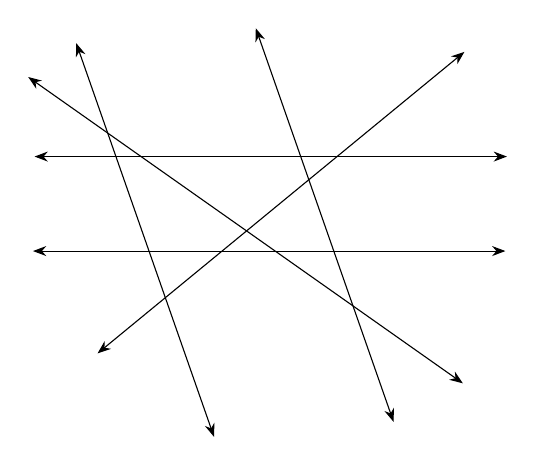
\begin{tikzpicture}[scale=1]
  % Coordinates
  \coordinate (A) at (0.94, 7.12);
  \coordinate (B) at (6.94, 7.12);
  \coordinate (D) at (0.92, 5.92);
  \coordinate (E) at (6.92, 5.92);
  \coordinate (C) at (6.40, 8.45);
  \coordinate (F) at (1.74, 4.62);
  \coordinate (G) at (3.75, 8.75);
  \coordinate (H) at (5.50, 3.75);
  \coordinate (I) at (0.86, 8.13);
  \coordinate (J) at (6.38, 4.24);
  \coordinate (K) at (1.47, 8.56);
  \coordinate (L) at (3.22, 3.56);

  % Drawing
  \draw[Stealth-Stealth] (A) -- (B);
  \draw[Stealth-Stealth] (D) -- (E);
  \draw[Stealth-Stealth] (C) -- (F);
  \draw[Stealth-Stealth] (G) -- (H);
  \draw[Stealth-Stealth] (I) -- (J);
  \draw[Stealth-Stealth] (K) -- (L);
\end{tikzpicture}
\caption{Two IZZes segment the plane into 20 regions}
\label{fizz:n2}
\end{figure}

\pagebreak
Now back to the original zig-zag to find $\zz_n$. The zig-zag is just like an IZZ, except each one creates four less regions. 
\[
\begin{tikzpicture}[scale=1]
  % Coordinates
  \coordinate (A) at (0.00, 6.00);
  \coordinate (B) at (5.00, 6.00);
  \coordinate (C) at (2.00, 4.00);
  \coordinate (D) at (7.00, 4.00);
  \coordinate (E) at (6.94, 7.19);
  \coordinate (F) at (7.03, 6.04);
  \coordinate (G) at (0.00, 2.75);
  \coordinate (H) at (0.00, 4.00);
  \coordinate (I) at (2.00, 6.67);
  \coordinate (J) at (1.45, 4.83);
  \coordinate (K) at (0.33, 3.23);
  \coordinate (L) at (2.73, 2.73);
  \coordinate (M) at (5.04, 4.72);
  \coordinate (N) at (6.66, 6.30);

  % Drawing
  \draw[Stealth-] (A) -- (B);
  \draw (B) -- (C);
  \draw[-Stealth] (C) -- (D);
  \draw[loosely dashed] (B) -- (E);
  \draw[loosely dashed] (B) -- (F);
  \draw[loosely dashed] (C) -- (G);
  \draw[loosely dashed] (C) -- (H);
  \node[above] at (I) {$1$};
  \node[above] at (J) {$2$};
  \node[above] at (K) {$\cancel3$};
  \node[above] at (L) {$\cancel4$};
  \node[above] at (M) {$\cancel5$};
  \node[above] at (N) {$\cancel6$};
\end{tikzpicture}
\]
So $n$ zig-zags will have $4n$ less regions than $n$ IZZes. That is,
\begin{align*}
\zz_n = {} & \infzz_n - 4n  \\
= {} & \frac{9}{2}n^2 + \frac{1}{2}n + 1 - \frac{8}{2}n && \showfrom{\eqref{fizz:selfcontained}}\\
= {} & \frac{9}{2}n^2 - \frac{7}{2}n + 1.
\end{align*}
\end{sol}

\end{document}
